\section{Discussion}
\label{sec:discussion}
The custom comparison holds channel widths, pooling schedule, training budget
and optimizer fixed, while Model B introduces depthwise/pointwise factorization
and additional normalization and ReLU operations. Thus the observed difference
cannot be attributed solely to the convolution operator. Both custom models
show validation fluctuations, making the saved best checkpoint preferable to
blindly using the final epoch.
The class-level errors explain why aggregate metrics should be read together.
In Figure~\ref{fig:model_a_cm}, 50 HerbaceousVegetation images are predicted as
PermanentCrop, contributing to PermanentCrop precision of
\APermanentPrecision\%. In Figure~\ref{fig:model_b_cm}, 22 Highway images are
predicted as Industrial; Highway recall is \BHighwayRecall\%. Model B thus
changes the error distribution rather than uniformly reducing performance.

In Figure~\ref{fig:mobilenet_v2_cm}, the largest directed confusion count is
10, shared by PermanentCrop predicted as HerbaceousVegetation and River
predicted as Highway. EfficientNet-B0's largest directed confusion is 14
AnnualCrop images predicted as PermanentCrop
(Figure~\ref{fig:efficientnet_b0_cm}). Crop categories may share colour and
texture at this resolution, but image-level analysis would be needed to
establish the causes. The matrices show which errors occur, not why they occur.

Figure~\ref{fig:representative-errors} shows two deterministic examples from
each of four measured Model A confusion directions. The crop pairs support the
matrix-level observation that some land-cover textures and long linear features
can appear similar at $64\times64$. They are examples of recorded errors, not
evidence that one visual feature caused every error.
\begin{figure}[H]\centering
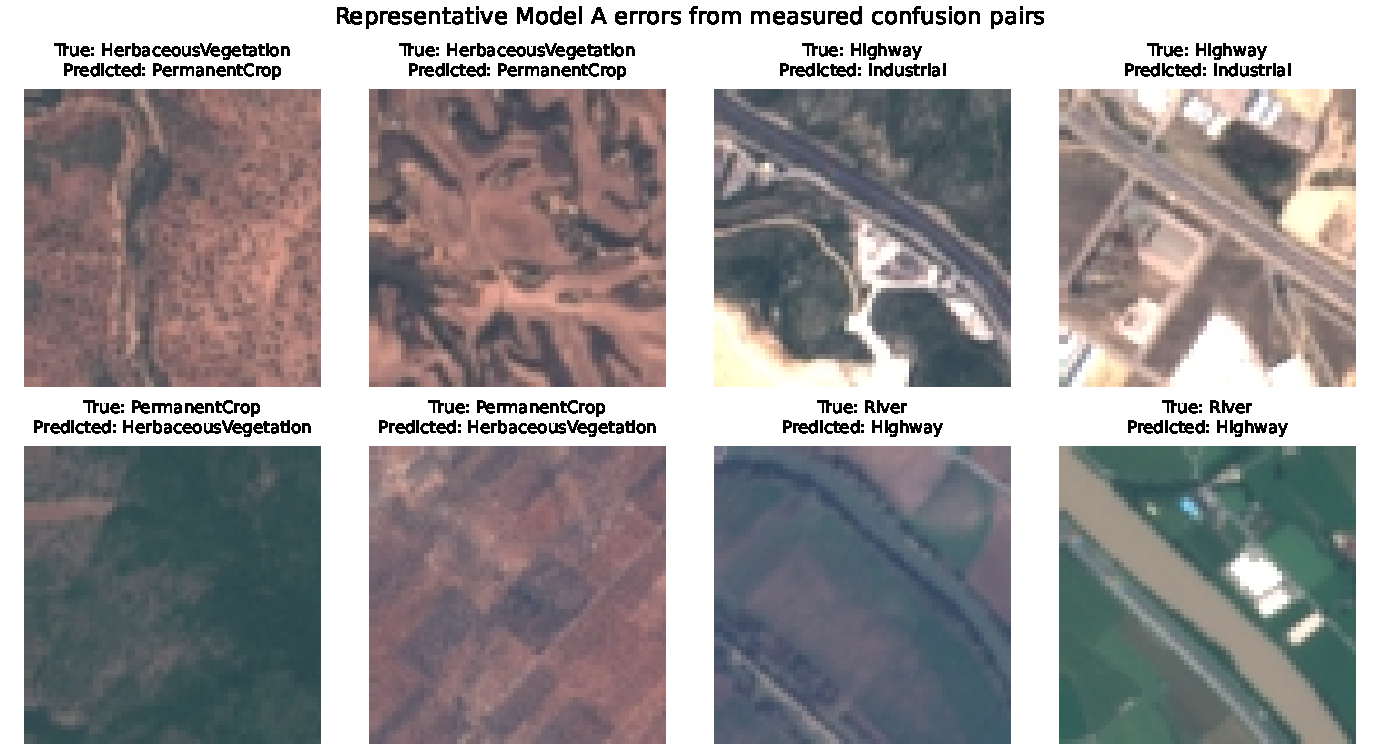
\includegraphics[width=\textwidth]{figures/representative_errors.pdf}
\caption{Representative Model A test errors selected from four confusion pairs.}
\label{fig:representative-errors}
\end{figure}

These are single-seed observations with no confidence intervals or repeated-run
variance estimate. Small accuracy differences should not be treated as proven
general advantages. The split is stratified but not geographic; satellite
scene correlation can make generalization to new regions harder than this
test suggests. ImageNet transfer supplies additional prior information, and
the 64x64 input differs from the pretrained recipe. These results are not the
best attainable performance of the pretrained architectures. The optimizer pilot compares
three fixed configurations for a short budget; it does not prove universal
optimizer superiority. No unseen edge device or energy benefit is asserted.

The deployment choice is therefore conditional. Model B is attractive when
weight storage is severe and a small accuracy loss is acceptable. MobileNetV2
is preferred when accuracy has priority and several MiB of weights are
acceptable. EfficientNet-B0 is not preferred here because it is less accurate,
larger and slower than MobileNetV2 under the tested setup. Before deployment,
the team would still need target-device peak RAM, quantized accuracy, operator
support, latency and power measurements.
